% !TeX root = ../tesis.tex

\chapter{Esparcimiento de luz por partículas}
\label{chapter:theory}

\vspace*{7em}

It is recommended to write a summary about the contents of this chapter as an introduction to them. 


\section{Fundamentos}
\label{section:basics}

La electrodinámica clásica es descrita mediante la fuerza de Lorentz y las ecuaciones de Maxwell \cite{griffithsIntroductionElectrodynamics2023}. En el sistema internacional de unidades, las ecuaciones de Maxwell en su forma diferencial están dadas por \cite{griffithsIntroductionElectrodynamics2023}
%
	\begin{subequations} \label{eqs:Maxwell}
	\begin{tcolorbox}[
	ams align, breakable]
	\nabla \cdot\vb{E} &= \frac{\rho_{tot}}{\varepsilon_0}, &\mbox{(Ley de Gauss eléctrica)}  
	\label{seq:GE} \\
	\nabla \cdot\vb{B} &= 0,						&\mbox{(Ley de Gauss magnética)}   
	\label{seq:GM} \\
	\nabla \times\vb{E} &= -\pdv{\vb{B}}{t}, 	&\mbox{(Ley de Faraday-Lenz)}		
	\label{seq:FL}\\
	\nabla \times\vb{B} &= \mu_0 \vb{J}_{tot} +\varepsilon_0\mu_0 \pdv{\vb{E}}{t}, &
	\mbox{(Ley de Ampère-Maxwell)} \label{seq:AM}
	\end{tcolorbox}\end{subequations}\noindent
%
donde $\vb{E}$ representa al campo eléctrico y $\vb{B}$ al campo magnético; $\rho_{tot}$ representa a la densidad de carga volumétrica y $\vb{J}_{tot}$ a la densidad de corriente volumétrica; $\epsilon_0$ a la permitividad eléctrica en el vacío y $\mu_0$ a la permeabilidad magnética en el vacío. Las ecuaciones de Maxwell pueden desacoplarse para obtener ecuaciones de segundo orden separadas para $\vb{E}$ y $\vb{B}$. En particular, al considerar un medio sin fuentes, es decir, $\rho_{tot}=0$ y $\vb{J}_{tot}=0$, y emplear la transformada de Fourier,  se obtiene que los campos electromagnéticos satisfacen la ecuación de onda vectorial~\cite{jacksonClassicalElectrodynamics2021}

	\begin{subequations}%
	\eqhalf{\nabla^2\vb{E} + k^2 \vb{E}=\vb{0},}%
	\eqhalf{\nabla^2\vb{B} + k^2 \vb{B}=\vb{0}.}\label{eq:Helmholtz}%
	\end{subequations}\vspace*{-1em}

\noindent Una de las posibles soluciones son las ondas planas expresadas como 

	\begin{subequations}%
	\eqhalf{\vb{E}(\vb{r},t) =\vb{E_0}e^{i(\vb{k}\cdot\vb{r} -\omega t)},}%
	\eqhalf{\vb{B}(\vb{r}, t) =\vb{B_0}e^{i(\vb{k}\cdot\vb{r} -\omega t)},}	
	\label{eqs:ondasPlanas}\end{subequations}\vspace*{-1em}
		
\noindent donde $\vb{E}_0$ y $\vb{B}_0$ corresponden a las amplitudes de los campos, $\omega$ la frecuencia angular de la onda y $\vb{k}$ el vector de onda. Para que se satisfagan las Ecs. \eqref{eqs:ondasPlanas}, se tiene que cumplir la relación de dispersión dada por $k=\sqrt{\mu\epsilon}\;\omega$, donde $\epsilon$ y $\mu$ corresponden a la permitividad eléctrica y la permeabilidad magnética del medio \cite{jacksonClassicalElectrodynamics2021}. La relación de dispersión se puede reescribir en términos del índice de refracción del material dado por
%
\begin{tcolorbox}[ams align]
	n(\omega) = \sqrt{\dfrac{\mu\varepsilon(\omega)}{\varepsilon_0 \mu_0}},
	\label{eq:indice} 
\end{tcolorbox}
%	
\noindent con lo que se obtiene,
%
\begin{tcolorbox}[ams align]
	k(\omega) = \sqrt{\dfrac{\omega\;c}{n(\omega)}},
	\label{eq:vector_onda} 
\end{tcolorbox}

\noindent donde $c=1/\sqrt{\epsilon_0\mu_0}$ es la velocidad de la luz en el vacío.

Al analizar la energía total almacenada en los campos electromagnéticos y el trabajo que estos realizan sobre una distribución de cargas y corrientes, se establece el teorema del trabajo y la energía. A partir de este teorema, se introduce el concepto de energía transportada por los campos por unidad de tiempo y por unidad de área, el cual está representado por el vector de Poynting, $\vb{S}$ \cite{griffithsIntroductionElectrodynamics2023}

\begin{tcolorbox}[ams align]
	\vb{S}=\frac{1}{\mu_0}(\vb{E}\times\vb{B}),
	\label{eq:vect_Poynting} 
\end{tcolorbox}

Las Ecs. \eqref{eqs:Maxwell} determinan los campos que surgen a partir de corrientes y cargas presentes en la materia. No obstante, dichas ecuaciones no explican el origen de estas corrientes y cargas. Por ello, es necesario complementarlas con ecuaciones llamadas \textit{relaciones constitutivas}, que describen cómo responde la materia ante la acción de los campos. Para un medio lineal, homogéneo e isótropo, las relaciones constitutivas están dadas por \cite{novotnyPrinciplesNanooptics2012}
%
\begin{subequations} \label{eqs:Constitutivas}
	\begin{tcolorbox}[
		ams align, breakable]
		\vb{D} &= \epsilon \vb{E}, \\
		\label{seq:D} 
		\vb{B} &= \mu \vb{H},\\
		\label{seq:B} 
		\vb{J} &= \sigma \vb{E}.
		\label{seq:J}\end{tcolorbox}\end{subequations}\noindent

A partir de la forma integral de las ecuaciones de Maxwell, se deducen las condiciones de frontera sobre los campos electromagnéticos al atravesar una interfaz entre dos medios distintos. Cada uno de los medios está caracterizado por una función dieléctrica y una permeabilidad magnética ($\epsilon_1, \mu_1$ para el medio 1 y $\epsilon_2, \mu_2$ para el medio 2). Para deducirlas, se considera un prisma de altura $\delta$ y área transversal $A$ [Fig. \ref{cond_perp}], y un circuito rectangular de altura $\delta$ y longitud $l$ [Fig. \ref{cond_par} ]. Bajo las suposiciones de medios lineales, homogéneos e isótropos, y en ausencia de fuentes externas ($\sigma_{\text{ext}} = 0$, $\vb{K}_{\text{ext}} = 0$), al emplear de las ecuaciones de Maxwell en su forma integral y las Ecs. \eqref{eqs:Constitutivas}, se obtienen a las siguientes condiciones de frontera:

%
\begin{subequations} \label{eqs:Constitutivas}
	\begin{tcolorbox}[
		ams align, breakable]
		\eqhalf{\epsilon_1E_1^{\perp}-\epsilon_2E_2^{\perp}= 0,}%
		\eqhalf{\vb{E}_1^{\parallel}-\vb{E}_1^{\parallel}=0,}\\
		\label{seq:D} 
		\eqhalf{B_1^{\perp}-B_2^{\perp}=0,}%
		\eqhalf{\frac{\vb{B}_1}{\mu_1}-\frac{\vb{B}_2}{\mu_2}=0,}		\label{seq:D} \end{tcolorbox}\end{subequations}\noindent

%
\begin{figure}[H]
	\centering
	\sidesubfloat[First image]{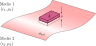
\includegraphics[width=0.4\textwidth]{../Figuras/condiciones_contorno_perp}\label{cond_perp}}
	\sidesubfloat[Second image]{\includegraphics[width=0.4\textwidth]{../Figuras/condiciones_contorno_par}\label{cond_par}}
	\caption{Esquema de una interfaz que separa dos medios distintos. El medio 1 se encuentra caracterizado por una función dieléctrica $\epsilon_1$ y una permeabilidad magnética $\mu_1$, mientras que el medio 2 se encuentra caracterizado por una función dieléctrica $\epsilon_2$ y una permeabilidad magnética $\mu_2$. \textbf{a)} Interfaz con una densidad superficial de carga $\rho_{tot}$ que es atravesada por un prisma rectangular de altura $\delta$ y área $A$. \textbf{b)} Interfaz con una densidad de superficial de corriente $\vb{K}_{tot}$. La densidad de corriente atraviesa una superficie rectangular de altura $\delta$ y longitud $l$.}
	\label{condiciones_frontera}
\end{figure}
%

La función dieléctrica y el índice de refracción del medio son en general, funciones complejas de la frecuencia de la forma \cite{maierPlasmonicsFundamentalsApplications2007}
%
	\begin{subequations} \label{eqs:n_epsilon}
	\begin{tcolorbox}[
		ams align, breakable]
		n(\omega) &= \eta + i\kappa,
		\label{seq:n} \\
		\epsilon(\omega) &= \epsilon_1 + i\epsilon_2, \label{seq:epsilon}
\end{tcolorbox}\end{subequations}
%
\noindent que se pueden determinar experimentalmente a través de mediciones de reflectancia y de la relación entre ambas dada por $n=\sqrt{\epsilon}$, de donde se obtiene \cite{maierPlasmonicsFundamentalsApplications2007}
\begin{align} \label{eqs:rel_n_epsilon}
		\epsilon_1 &= \eta^2 - \kappa^2, \\
		\label{seq:eps1} 
		\epsilon_2 &=2\eta\kappa,\\
		\label{seq:eps2} 
		\eta^2&=\frac{\epsilon_1}{2}+\frac{1}{2}\sqrt{\epsilon_1^2+\epsilon_2^2},\\
		\label{seq:eta}
		\kappa &=\frac{\epsilon_2}{2\eta},
		\label{seq:kappa}
\end{align}
donde $\kappa$ es llamado el coeficiente de extinción y determina la absorción óptica de las ondas electromagnéticas propagándose a través del medio \cite{maierPlasmonicsFundamentalsApplications2007}.  


Como la respuesta óptica de los materiales depende en general de la frecuencia, se tiene que tomar en cuenta la no localidad en el tiempo y espacio al generalizar las Ecs. anteriores como:
%

